\section{Introduction}

%Tracing algorithms is ubiquitous, fundamental
Tracing algorithms on examples is fundamental to how teachers and students in
computer science explain and learn. On the blackboard, teachers explain an
algorithm for the first time by drawing an example data structure and carrying
out the algorithm's operation on the example. Similarly, before diving into
coding and problem sets, students review algorithms by reading pseudocode and
tracing through multiple examples on paper.
% mentally tracing the algorithm's behavior

% Tedious, limiting no manipulation affordances no persistent, structured
% recording
This process of tracing algorithms on blackboards and paper can be tedious and
limiting. First, blackboards and paper do not afford manipulation of the
drawing: in order to demonstrate changes, the user must erase, redraw, and
storyboard the behavior as a series of snapshots.
Second, the drawing is not recorded in a persistent, structured format, so it
can be difficult for students and teachers to share ideas and discuss problems.
This is particularly problematic in a MOOC context, where the majority of
students do not have access to teaching staff.

\begin{figure}

\begin{center}
%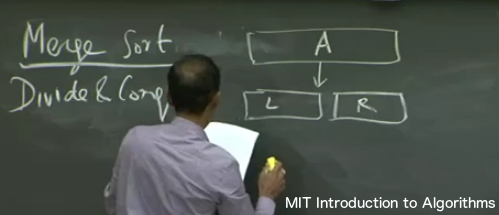
\includegraphics[width=0.55\columnwidth]{img/frontpage-6006.png}
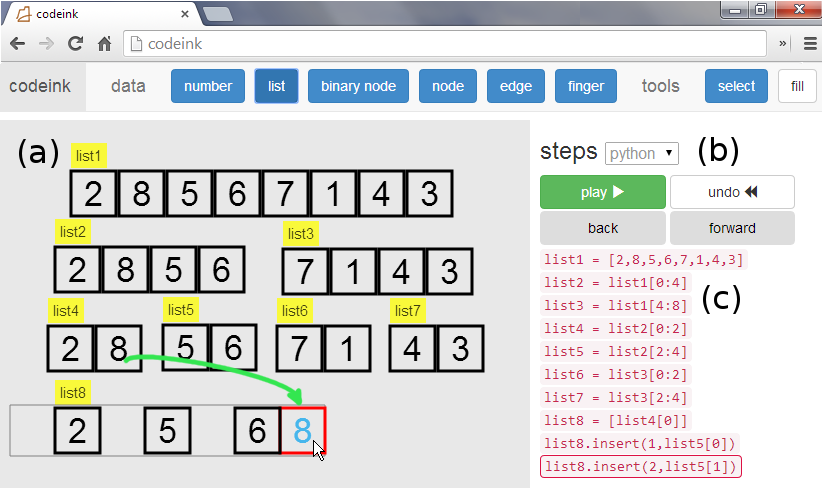
\includegraphics[width=\columnwidth]{img/frontpage-mergesort.png}
\end{center}

\vspace{-0.5em}

\caption{CodeInk is a Web-based tool that implements a direct
manipulation language for tracing algorithms on data structures for the
purpose of CS education. CodeInk allows the user to (a) compose and
manipulate data structures on a graphical canvas, (b) step forward and
backward through the recorded trace, and (c) see each step translated
into a line of Python code or an English explanation.}

%The CodeInk user interface is (a) a canvas for composing and
%manipulating data structures and (c) an interactive list of Python steps
%recorded by the tool, based on the user's interactions. The user can
%step forward and backward through the steps, or replay the entire trace
%using the playback controls (b).}

\label{fig:codeink-intro}
\end{figure}

% Code-driven visualization is for visualization, not explanation or active
% learning Also at the wrong level of abstraction
Code-driven visualization offers an alternative to tracing-by-drawing, where the
user can input an algorithm's code and watch an animation of its execution.
However, watching visualizations is a passive learning process, where tracing
requires the student to play the role of the computer and actively carry out the
algorithm's behavior. Moreover, an algorithm's code is usually at a lower level
of abstraction (language and implementation specific) than the one at which the
algorithm should be explained and learned (language and implementation
agnostic).

We present CodeInk, a CS education tool designed to reduce the tedium and
enhance the experience of tracing algorithms. Using a direct manipulation (DM)
gesture set, users can demonstrate changes to data structures, rather than draw
before and after snapshots. The trace is recorded as an interactive set of
program steps, where each gesture is translated to a line of Python code or
explanatory English. The steps provide several benefits: feedback on user
interactions, navigation through the trace, and a persistent, structured format
that can be easily disseminated and analyzed as a basis for discussion.

For example, an instructor can explain merge sort by dragging an example list
onto the canvas, selecting sublists with a rectangular selection, dragging them
away to create copies, then merging elements by dragging them into a new sorted
list (\fig{fig:codeink-intro}a). Every interaction is interpreted as a step in
Python (\fig{fig:codeink-intro}c). The trace can then be shared with students,
who can navigate through the explanation by clicking on steps
(\fig{fig:codeink-intro}b), and then trace the algorithm for themselves on a new
example. Their own trace can be shared with teachers as a basis for feedback on
not just the final output, but also the process by which the list was sorted.

%We have built CodeInk, a system that enables teachers and students to trace an
%algorithm's behavior by directly manipulating visual objects on a stage. The
%objects represent data structures as they are typically drawn (lists, trees,
%graphs) and can be manipulated using a set of DM gestures to demonstrate
%concrete changes to values and pointer assignments. CodeInk translates all
%interactions into a list of steps, which can be used to navigate through the
%algorithm's trace. In the case where a student is tracing the algorithm's
%behavior, the steps capture their understanding in a structured format, making
%the demonstration analyzable where screencasts, and audio/video recordings are
%not.

This paper makes the following primary contributions:

\begin{enumerate} %\itemsep1pt

\item CodeInk: a CS education tool that enhances the experience of tracing
algorithms on example data structures.
\item A direct manipulation (DM) gesture set for demonstrating changes to list,
tree and graph data structures, where each gesture maps onto a line of Python
code.
\item An evaluation of CodeInk's usability and viability in a controlled study,
where students watched CodeInk-produced traces to learn an algorithm, then used
CodeInk to trace the algorithm for themselves to solidify their
understanding.

\end{enumerate}

